% !TEX encoding = UTF-8 Unicode
\documentclass[12pt,a4paper]{report}
 
\usepackage[brazil]{babel}
\usepackage[utf8]{inputenc}
\usepackage[T1]{fontenc}
\usepackage{graphicx}
\usepackage{listings}
\usepackage{color}

\definecolor{mygreen}{rgb}{0,0.6,0}
\definecolor{mygray}{rgb}{0.5,0.5,0.5}
\definecolor{mymauve}{rgb}{0.58,0,0.82}

\lstset{ %
  backgroundcolor=\color{white},   % choose the background color; you must add \usepackage{color} or \usepackage{xcolor}
  basicstyle=\footnotesize,        % the size of the fonts that are used for the code
  breakatwhitespace=false,         % sets if automatic breaks should only happen at whitespace
  breaklines=true,                 % sets automatic line breaking
  captionpos=b,                    % sets the caption-position to bottom
  commentstyle=\color{mygreen},    % comment style
  deletekeywords={...},            % if you want to delete keywords from the given language
  escapeinside={\%*}{*)},          % if you want to add LaTeX within your code
  extendedchars=true,              % lets you use non-ASCII characters; for 8-bits encodings only, does not work with UTF-8
  frame=single,                    % adds a frame around the code
  keywordstyle=\color{blue},       % keyword style
  language=Octave,                 % the language of the code
  morekeywords={*,...},            % if you want to add more keywords to the set
  numbers=left,                    % where to put the line-numbers; possible values are (none, left, right)
  numbersep=5pt,                   % how far the line-numbers are from the code
  numberstyle=\tiny\color{mygray}, % the style that is used for the line-numbers
  rulecolor=\color{black},         % if not set, the frame-color may be changed on line-breaks within not-black text (e.g. comments (green here))
  showspaces=false,                % show spaces everywhere adding particular underscores; it overrides 'showstringspaces'
  showstringspaces=false,          % underline spaces within strings only
  showtabs=false,                  % show tabs within strings adding particular underscores
  stepnumber=2,                    % the step between two line-numbers. If it's 1, each line will be numbered
  stringstyle=\color{mymauve},     % string literal style
  tabsize=2,                       % sets default tabsize to 2 spaces
  title=\lstname                   % show the filename of files included with \lstinputlisting; also try caption instead of title
}
\renewcommand*{\lstlistingname}{Exemplo}

\graphicspath{ {images/} }

\title{Solução para captura de análise de sinais analógicos}
\author{Alves, M.\\
	\and
	de Araújo, V.\\
	\and
	Lenza, T.\\
	\and
	Pedreira, M.\\
	\and
	Sandoval, D. A. M.\\
	daniel@loopec.com.br}
\begin{document}
\maketitle
\tableofcontents

\chapter{Introdução}

% Inserir introdução sobre a importância de sinais analógicos e da capacidade de estudá-los

\section{Objetivos}

% Inserir objetivos almejados ao realizar o trabalho

\section{Sinais Analógicos}

%Base de todos os sistemas de telecomunicações;
%Sinais mecânicos: som, sensores;
%Sinais eletromagnéticos: Wi-Fi, Bluetooth, AM, FM, rede elétrica.

\subsection{Transmissão de Dados}

%Dados digitais são modulados em sinais analógicos para transmissão;
%Maior robustez à interferência e atenuação.

\chapter{Projeto de Hardware}
\lstinputlisting[language=C,caption={Código do Arduino},label={lst:arduino}]{code/arduino.c}

%Aquisição do sinal analógico
%	•	Convertido em sinal elétrico, caso não o seja;
%	•	Amostrado e quantizado;
%Arduino Uno
%	•	Plataforma de desenvolvimento de hardware;
%	•	Baseado no ATmega328;
%	•	2KB SRAM, 1KB EEPROM, 16MHz.
%Aquisição com Arduino
%	•	Detecta variações entre 0-5V;
%	•	1024 níveis;
%	•	800 leituras, a 470Hz.
%	•	Teorema de Nyquist:
%	•	Podemos amostrar sinais de até 235Hz com a taxa de amostragem 470Hz.

\begin{figure}[p]
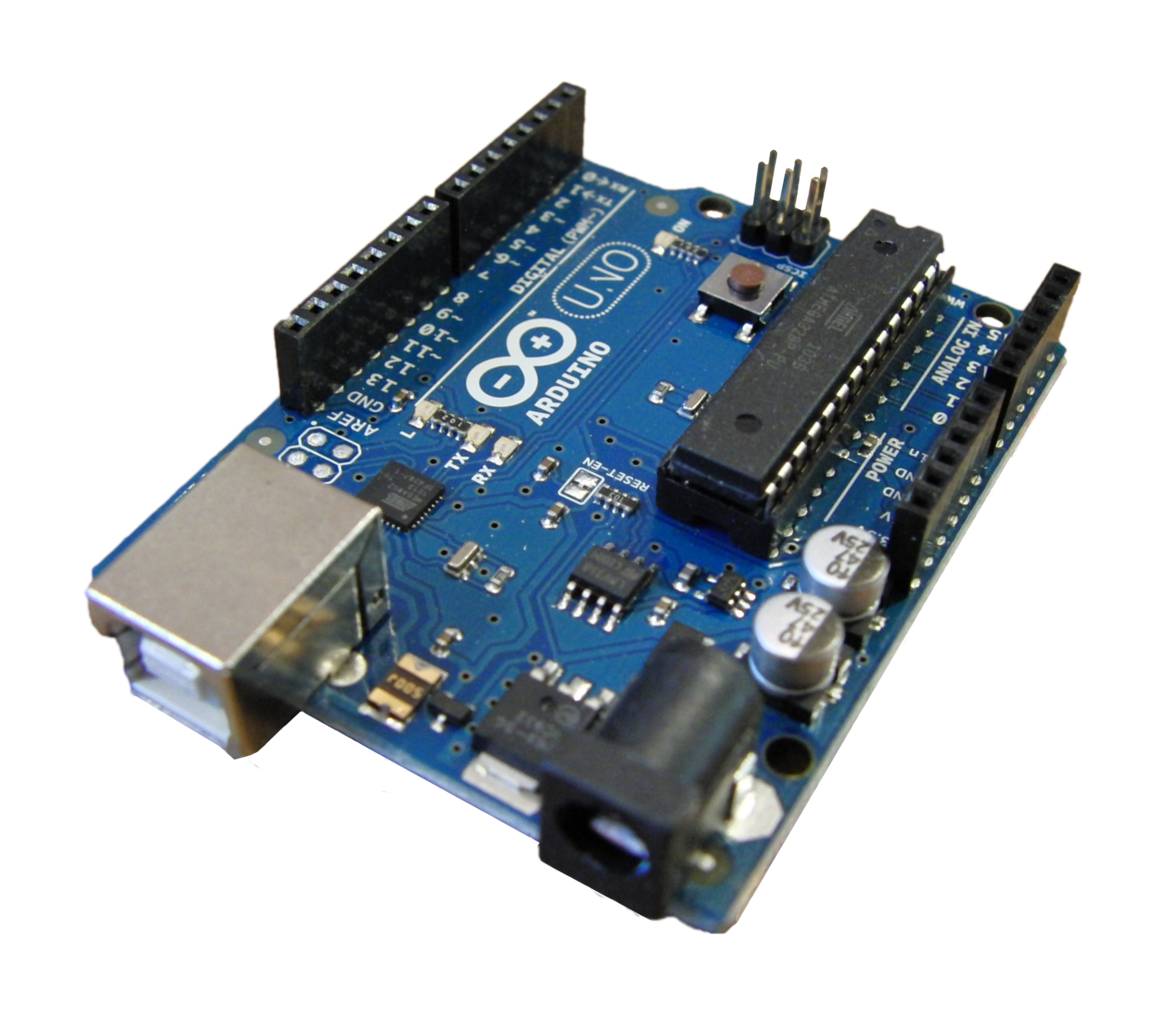
\includegraphics[width=0.8\textwidth]{arduino.png}
\caption{Arduino Uno}
\label{fig:arduino}
\end{figure}

\chapter{Projeto de Software}

%Análise do Sinal
%	•	Recepção dos dados via interface Serial;
%	•	Análise no domínio da frequência;
%	•	Visualização gráfica dos resultados.
%Série de Fourier
%	•	Todo sinal pode ser representado por uma soma de senos e cossenos, denominada Série de Fourier.
%Análise no domínio da frequência
%	•	Sinal é decomposto em sinais periódicos de diferentes amplitudes;
%	•	Transformada rápida de fourier (FFT);
%	•	Observamos a magnitude em cada frequência separadamente.
%INCLUIR INFORMAÇÕES SOBRE PROJETO DO SOFTWARE DE CÁLCULO DA INTEGRAL

\chapter{Resultados}

%Incluir imagens e discutir resultados obtidos.

\end{document}
